\documentclass[man]{apa6}

\usepackage{amssymb,amsmath}
\usepackage{ifxetex,ifluatex}
\usepackage{fixltx2e} % provides \textsubscript
\ifnum 0\ifxetex 1\fi\ifluatex 1\fi=0 % if pdftex
  \usepackage[T1]{fontenc}
  \usepackage[utf8]{inputenc}
\else % if luatex or xelatex
  \ifxetex
    \usepackage{mathspec}
    \usepackage{xltxtra,xunicode}
  \else
    \usepackage{fontspec}
  \fi
  \defaultfontfeatures{Mapping=tex-text,Scale=MatchLowercase}
  \newcommand{\euro}{€}
\fi
% use upquote if available, for straight quotes in verbatim environments
\IfFileExists{upquote.sty}{\usepackage{upquote}}{}
% use microtype if available
\IfFileExists{microtype.sty}{\usepackage{microtype}}{}

% Table formatting
\usepackage{longtable, booktabs}
\usepackage{lscape}
% \usepackage[counterclockwise]{rotating}   % Landscape page setup for large tables
\usepackage{multirow}		% Table styling
\usepackage{tabularx}		% Control Column width
\usepackage[flushleft]{threeparttable}	% Allows for three part tables with a specified notes section
\usepackage{threeparttablex}            % Lets threeparttable work with longtable

% Create new environments so endfloat can handle them
% \newenvironment{ltable}
%   {\begin{landscape}\begin{center}\begin{threeparttable}}
%   {\end{threeparttable}\end{center}\end{landscape}}

\newenvironment{lltable}
  {\begin{landscape}\begin{center}\begin{ThreePartTable}}
  {\end{ThreePartTable}\end{center}\end{landscape}}

  \usepackage{ifthen} % Only add declarations when endfloat package is loaded
  \ifthenelse{\equal{\string man}{\string man}}{%
   \DeclareDelayedFloatFlavor{ThreePartTable}{table} % Make endfloat play with longtable
   % \DeclareDelayedFloatFlavor{ltable}{table} % Make endfloat play with lscape
   \DeclareDelayedFloatFlavor{lltable}{table} % Make endfloat play with lscape & longtable
  }{}%



% The following enables adjusting longtable caption width to table width
% Solution found at http://golatex.de/longtable-mit-caption-so-breit-wie-die-tabelle-t15767.html
\makeatletter
\newcommand\LastLTentrywidth{1em}
\newlength\longtablewidth
\setlength{\longtablewidth}{1in}
\newcommand\getlongtablewidth{%
 \begingroup
  \ifcsname LT@\roman{LT@tables}\endcsname
  \global\longtablewidth=0pt
  \renewcommand\LT@entry[2]{\global\advance\longtablewidth by ##2\relax\gdef\LastLTentrywidth{##2}}%
  \@nameuse{LT@\roman{LT@tables}}%
  \fi
\endgroup}


\ifxetex
  \usepackage[setpagesize=false, % page size defined by xetex
              unicode=false, % unicode breaks when used with xetex
              xetex]{hyperref}
\else
  \usepackage[unicode=true]{hyperref}
\fi
\hypersetup{breaklinks=true,
            pdfauthor={},
            pdftitle={Cue Weighting in L2 Stress Perception},
            colorlinks=true,
            citecolor=blue,
            urlcolor=blue,
            linkcolor=black,
            pdfborder={0 0 0}}
\urlstyle{same}  % don't use monospace font for urls

\setlength{\parindent}{0pt}
%\setlength{\parskip}{0pt plus 0pt minus 0pt}

\setlength{\emergencystretch}{3em}  % prevent overfull lines


% Manuscript styling
\captionsetup{font=singlespacing,justification=justified}
\usepackage{csquotes}
\usepackage{upgreek}



\usepackage{tikz} % Variable definition to generate author note

% fix for \tightlist problem in pandoc 1.14
\providecommand{\tightlist}{%
  \setlength{\itemsep}{0pt}\setlength{\parskip}{0pt}}

% Essential manuscript parts
  \title{Cue Weighting in L2 Stress Perception}

  \shorttitle{Spanish Stress}


  \author{Jessyca Campos\textsuperscript{1}}

  % \def\affdep{{""}}%
  % \def\affcity{{""}}%

  \affiliation{
    \vspace{0.5cm}
          \textsuperscript{1} Rutgers University\\
          \textsuperscript{}   }

  \authornote{
    Correspondence concerning this article should be addressed to Jessyca
    Campos, . E-mail:
    \href{mailto:jac706@rutgers.edu}{\nolinkurl{jac706@rutgers.edu}}
  }


  




\usepackage{amsthm}
\newtheorem{theorem}{Theorem}[section]
\newtheorem{lemma}{Lemma}[section]
\theoremstyle{definition}
\newtheorem{definition}{Definition}[section]
\newtheorem{corollary}{Corollary}[section]
\newtheorem{proposition}{Proposition}[section]
\theoremstyle{definition}
\newtheorem{example}{Example}[section]
\theoremstyle{definition}
\newtheorem{exercise}{Exercise}[section]
\theoremstyle{remark}
\newtheorem*{remark}{Remark}
\newtheorem*{solution}{Solution}
\begin{document}

\maketitle

\setcounter{secnumdepth}{0}



\section{Introduction}\label{introduction}

The goal of this study is to analyze the influence of syllable weight on
the perception of stress by late L2 learners of Spanish. How do late L2
learners of Spanish decide where to place lexical stress in the absence
of acoustic cues? The hypothesis being tested is that late learners will
rely on the weight of the syllable to aid them in perceiving stressed
syllables. As proficiency increases in the L2, the perception of
stressed syllables becomes more and more native-like, therefore, we
expect a positive correlation between a learner's proficiency and their
ability to perceive the correct stressed syllable. The overarching
question driving this study is: to what extent does the phonological
structure of language influence speech perception? (adopted from Hume \&
Johnson (1999)). We expect the late learner to become more attuned to
the unmarked Spanish stress patterns as they become more proficient in
the language.

To test the effects of syllable weight on stress perception an
experiment was designed in which disyllabic nonce words were created and
synthesized. Three nonce word used in the study, \emph{fafa},
\emph{fufu}, and \emph{fafal}. The data of interest in this experiment
were those in which acoustic correlates were neutral in regard to stress
in \emph{fafa} and \emph{fafal}. We will be comparing the proportion of
oxytone responses provided by participants for each of the two
conditions ( \emph{fafa}, \emph{fafal}) based on the participants
proficiency in Spanish.

\section{Methods}\label{methods}

\subsection{Participants}\label{participants}

68 subjects took part in this study. The subjects that took part in the
study were second language learners of Spanish of varying proficiencies
from Middleberry College. Participants did not know the purpose of the
study before beginning the experiment but were informed afterwards if
they were interested. None of the participants had any language or
hearing impairments.

\subsection{Stimuli}\label{stimuli}

The stimuli in this study were modified natural recordings of the words
\emph{fafa}, \emph{fufu}, and \emph{fafal} produced by a female speaker
then manipulated in Praat (Boersma \& Weenink, 2016). The nonce words
were chosen for this study because they do not violate any phonological
constraints in either Spanish or English. Combinations of different
measures of duration and intensity were created for each of the words
which produced stressed syllables that were either clear paroxytone,
paroxytone, neutral, oxytone, or clear oxytone (see Llebraria \& Prieto
(2016) for a detailed explanation of how the stimuli were manipulated).
There were a total of 25 different combinations of duration and
intensity for each word. In all, the participants heard 300 words during
the course of the experiment (25 variations x 3 words x 4 repetitions =
300 total). Although other stimuli were presented to the participants
during the experiment, this study focuses on the data where the
intensity and duration were 0. It is also important to note that the
words were said in isolation to ensure that the experiment was solely
analyzing lexical stress and not influenced by pitch accents.

\subsection{Procedure}\label{procedure}

Upon completing a proficiency test, the participants completed a
two-alternative forced choice task on a computer implemented through the
PyschoPy II software (Pierce 2009), in which they were asked to identify
the location of stress (first or second syllable) in disyllabic nonce
words \emph{fafa}, \emph{fufu}, and \emph{fafal} by clicking the
\enquote{1} or \enquote{0} keys on the keyboard. The participants were
instructed to wear headphones and select \enquote{1} if they perceived
the stress to fall on the first syllable of the word and \enquote{0} if
they thought stress fell on the second syllable. The participants heard
the audio stimuli while the words were displayed on the screen with the
first or second syllable capitalized (denoting the stressed syllable) on
the right-hand or left-hand side. The order in which the words were
presented to the participants was randomly assigned. The participant
needed to complete the cycle of the randomly assigned word (25
variations x 1 word x 4 repetitions) before moving forward to the other
words. They were offered a break at the end of each cycle. The average
time to complete the experiment was 20 minutes. The results of the
proficiency test and perception experiment were recorded by the computer
and collected at the end of the experiment.

\section{Results}\label{results}

The results of the experiment were compiled and analyzed in R. We used R
(Version 3.4.3; R Core Team, 2017) and the R-package \emph{papaja}
(Version 0.1.0.9709; Aust \& Barth, 2018) for all our analyses. The
packages \emph{Tidyverse()} (Wickham 2016) and \emph{rsq()} (Zhang 2017)
were also used.

The data was analyzed using a general linear model to see if the
proportion of oxytone responses differed as a function of condition (
\emph{fafa}/ \emph{fafal}) and proficiency. The model included
proportion of oxytone responses as the dependent variable, and condition
( \emph{fafa}/ \emph{fafal}) and proficiency as the independent
variables. A \emph{fafal} response was coded as \enquote{1} and a
\emph{fafa} response was coded as \enquote{0.} The data was centered by
proficiency. Significance of main effects and interactions were assessed
using hierarchical partitioning of the variance via nested model
comparisons. A visual inspection of Q-Q plots indicate that the
residuals are normally distributed. Other model diagnostics concluded
that the mean of residuals is zero and were homoscedastic, there were no
autocorrelation of residuals. Experiment-wise alpha was set at 0.05.

The plot shows the proportion of Oxytone responses as a function of
proficiency (centered) and condition ( \emph{fafa}, \emph{fafal}).

\begin{figure}

{\centering 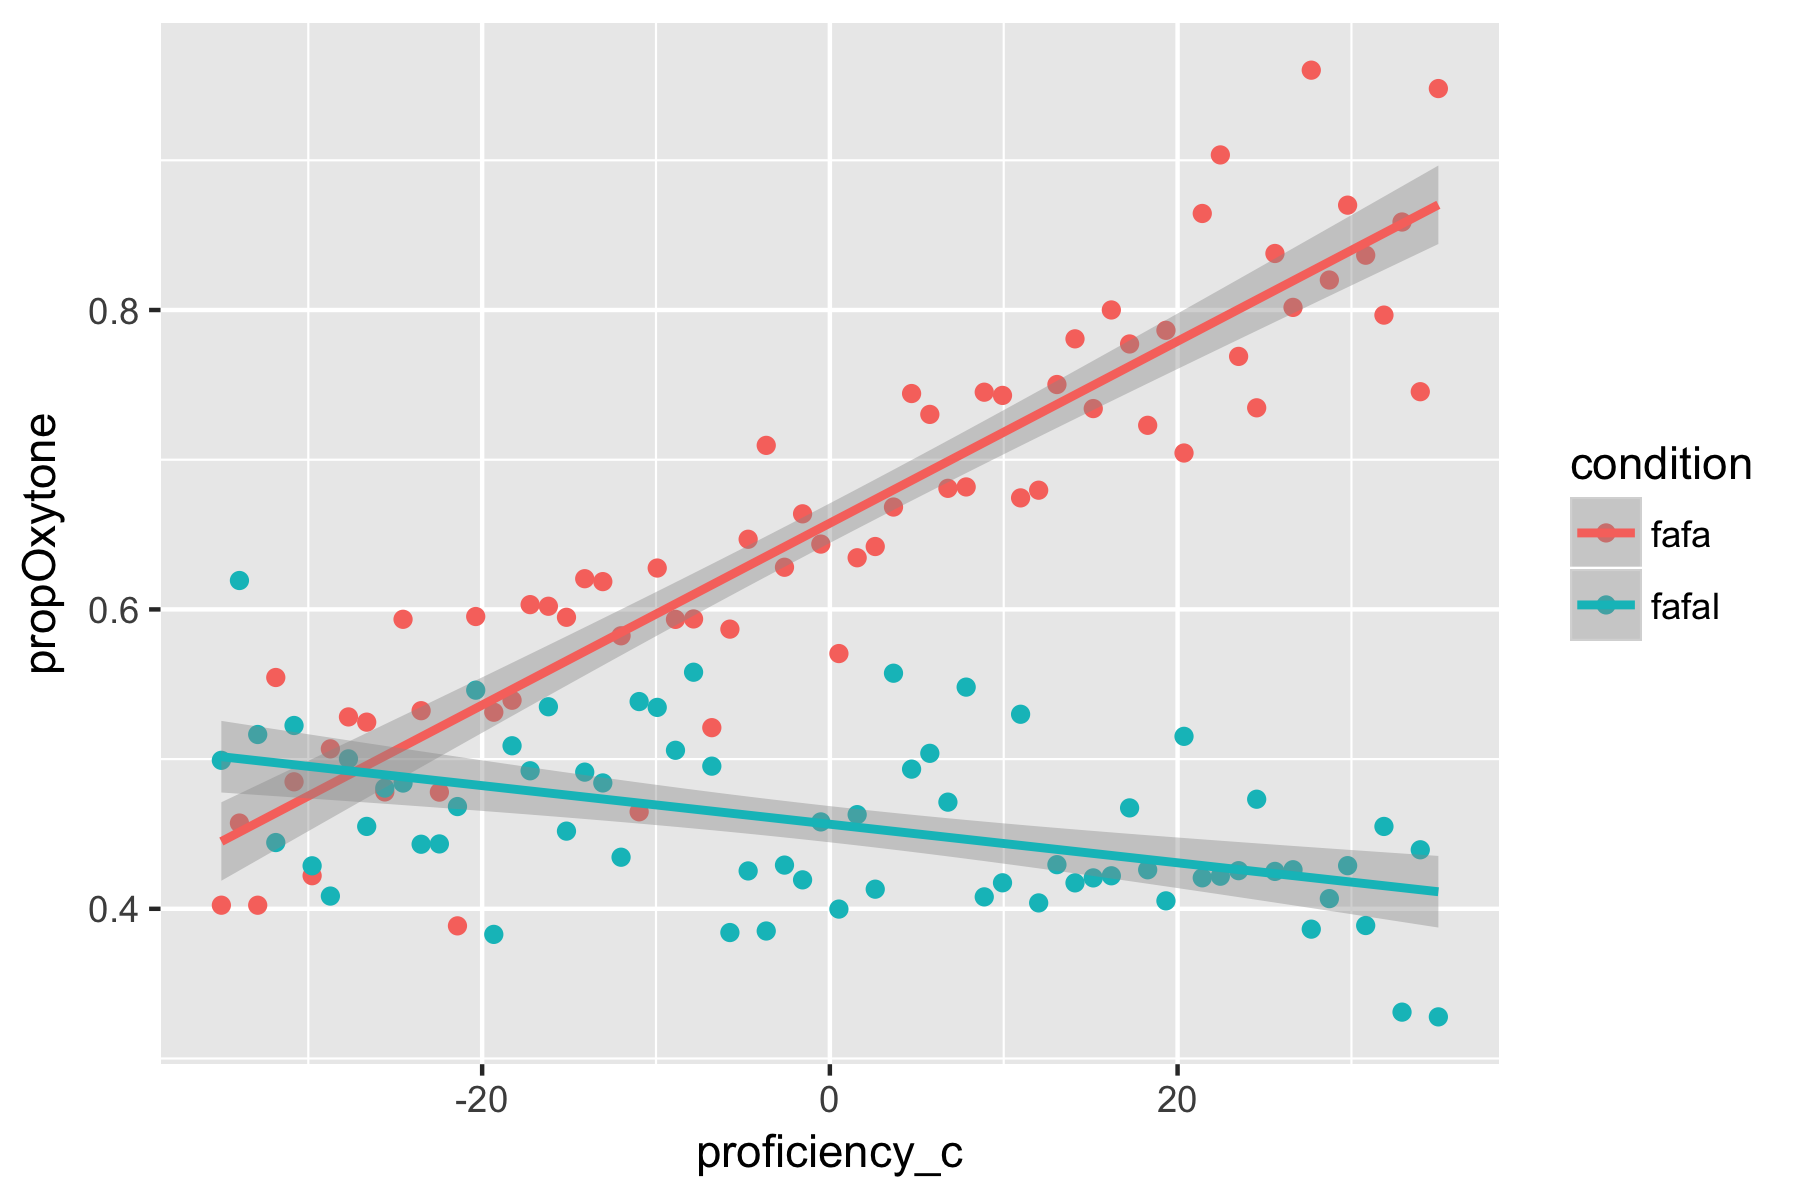
\includegraphics[width=450px,height=350px]{../figs/span_stress6x4} 

}

\caption{ }\label{fig:unnamed-chunk-1}
\end{figure}

The model revealed a main effect of \emph{proficiency}
{[}\(\chi\)\^{}2(1)= 0.3277; p\textless{} 0.01{]} and of
\emph{condition} {[}\(\chi\)\^{}2(1)= 1.3752; p\textless{} 0.01{]}.
There was a \emph{proficiency x condition} interaction
{[}\(\chi\)\^{}2(1)= 0.7756; p\textless{} 0.01{]} which makes
interpreting the main effects challenging. Visual inspection of the plot
suggests that the \emph{fafal} condition had higher values than the
\emph{fafa} condition. The best model was the model with the
\emph{condition x proficiency} interaction, 87.24\% of the variance in
the predictors in this model were accounted for by the response variable
{[}R\^{}2 = 0.8724{]}. Due to an error in coding the propOxytone
responses, the values for the \emph{fafa} condition correspond to those
of the \emph{fafal} condition and vice versa. There was a negative
correlation between the \emph{fafa} condition and proficiency; as
proficiency increased, participants were less likely to perceive the
word as being stressed on the first syllable (paroxytone) {[}\(\beta\) =
-0.2011; CI = -0.2187, -0.1835; SE = 0.0089; p \textless{} 0.001{]}. On
the contrary, there was a positive relationship between the \emph{fafal}
condition and the proportion of oxytone responses; as proficiency
increased participants were more likely to perceive stress on the final
syllable {[}\(\beta\) = 0.6576; CI = 0.6452, 0.6701; SE = 0.0064; p
\textless{} 0.001{]}. The model revealed that when confronted with
disyllabic nonce words in Spanish, late learners complied with the
unmarked stress patterns and perceived stress on the first syllable if
the syllable was light and stress on the final syllable if the final
syllable was heavy. Results of this analysis indicate that syllable
weight is a determiner in the perception of stress by late learners of
Spanish.

\section{Discussion}\label{discussion}

Findings support the hypothesis that late learners of Spanish use the
weight of the syllable in the absence of acoustic cues to aid in the
perception of stress. This was shown to be in true for both conditions (
\emph{fafa}, \emph{fafal}). As proficiency increased the proportion of
oxytone responses increased when the final syllable was heavy, in other
words, learners perceived the final syllable to be stressed when the
final syllable was heavy. We also saw that as proficiency increased the
proportion of oxytone responses decreased in disyllabic words with light
syllables.

When presented with an unfamiliar word, late learners will use
analogies, words in their L1 or L2 that share similar phonological or
morphological features to the unfamiliar word, to guide them in
emphasizing the correct syllable. Novice leaners tend to revert to their
L1 when looking for analogies while more experienced learners use their
L2 since their lexicon is more developed. The errors novice learners
make in finding analogies in their L1 is due to the fact that their
predictions of stress placement in the target language are based on
rules and constraints of their native language. Novice English-speaking
learners of Spanish have been shown to revert to their L1 stress system
which lead them to predict antepenultimate stress since the default
stress pattern in English is to stress the antepenultimate syllable
(Bullock and Lord 2003). As proficiency increases the learner becomes
more attuned to the unmarked stressed patterns of their L2, which, in
Spanish, is to stress the penultimate syllable in words that have light
final syllables and the final syllable in words that have a heavy final
syllable.

The second half of this discussion is more theoretically driven. The
overarching question driving this study was: to what extent does the
phonological structure of language influence speech perception? Syllable
weight influencing the perception of stress by late learners of Spanish
shows that phonological structure of language influences speech
perception to an extent. Further, the acquisition of Spanish Stress
rules by non-native speakers can be analyzed in terms of Optimality
Theory. In terms of OT, the faithfulness constraints that the language
is bound to follow and violate are the suprasegmental features such as
fundamental frequency (F0), duration, intensity, and vowel spectra.
Syllable weight is argued to be another constraint in a language that is
dominated by the acoustic correlates of stress. The unmarked structure
will emerge when the other acoustic correlates are neutralized leaving
the candidates to either remain faithful or violate the syllable weight
constraint. It is important to note that the acoustic correlates of
stress need to be absent in order to study the effect syllable weight
has on perception. If syllable weight were a constraint the language
needed to be faithful to, the ranking of the constraint would be
dominated by the acoustic correlates that have been proven to indicate
stress. This would mean that the unmarked rules in Spanish emerge
through the role of syllable weight in stress perception.

\section{Conclusion}\label{conclusion}

The present study examined the influence of syllable weight on the
perception of stress by late learners of Spanish. Findings support the
hypothesis that late learners of Spanish use the weight of the syllable
in the absence of acoustic cues. This suggests that as a learner's
proficiency increases they are becoming more attuned to the unmarked
stress patterns in Spanish. This is important because it supports the
claim that phonological structure of language influences speech
perception.

\newpage

\section{References}\label{references}

Aske, J. (1990). Disembodied rules versus patterns in the lexicon:
Testing the psychological reality of Spanish stress rules. In K. Hall,
J. P. Koenig, M. Meacham, S. Reinman, \& L. A. Sutton (Eds.),
Proceedings of the Sixteenth Annual Meeting of the Berkeley Linguistics
Society (pp.~30-45).

Aust, F., \& Barth, M. (2018). papaja: Create APA manuscripts with R
Markdown. Retrieved from \url{https://github.com/crsh/papaja}

Bullock, B., \& Lord, G. (2003). Analogy as a learning tool in second
language acquisition: The case of Spanish stress. Amsterdam studies in
the theory and history of linguistic science, 281-297.

Chrabaszcz, A., Winn, M., Lin, C. Y., \& Idsardi, W. J. (2014). Acoustic
cues to perception of word stress by English, Mandarin, and Russian
speakers. Journal of Speech, Language, and Hearing Research, 57(4),
1468-1479.

Face, T. L. (2000). The role of syllable weight in the perception of
Spanish stress. In H. Campos, E.Herburger, A. Morales-Front, \& T. J.
Walsh (Eds.), Hispanic linguistics at the turn of the millennium
(pp.~1-13). Somerville, MA: Cascadilla Proceedings Project.

Face, T. L. (2005). Syllable weight and the perception of Spanish stress
placement by second language learners. Journal of Language and Learning,
3(1), 90-103.

Peirce, JW (2009) Generating stimuli for neuroscience using PsychoPy.
Front. Neuroinform. 2:10. \url{doi:10.3389/neuro.11.010.2008}

R Core Team. (2017). R: A language and environment for statistical
computing. Vienna, Austria: R Foundation for Statistical Computing.
Retrieved from \url{https://www.R-project.org/}

\begingroup
\setlength{\parindent}{-0.5in} \setlength{\leftskip}{0.5in}

\hypertarget{refs}{}
\hypertarget{ref-R-papaja}{}
Aust, F., \& Barth, M. (2018). \emph{papaja: Create APA manuscripts with
R Markdown}. Retrieved from \url{https://github.com/crsh/papaja}

\hypertarget{ref-R-base}{}
R Core Team. (2017). \emph{R: A language and environment for statistical
computing}. Vienna, Austria: R Foundation for Statistical Computing.
Retrieved from \url{https://www.R-project.org/}

\endgroup






\end{document}
